\section{GAMYGDALA}
In the Gamygdala world, Agents have goals they want to achieve. Based on their beliefs, they assess whether or not they have achieved their goals, and for example what's the likelihood to achieve their goals. Based on these properties and based on the relation with other agents, the agent's emotion is calculated. \\ 

Each Agent has a separate Goal base which they update every evaluation cycle. Whenever an event happens, the impact on a particular goal has to be provided. New agent-specific values like the goal likelihood, change in likelihood, the overall utility of the goal (how useful is it to achieve the goal) are then recalculated. Finally, a new emotion is distilled from all these particular properties. \\

Because each goal is unique and interchangeable, the engine itself also keeps track of all goals. \\

In this section, first you will get insight into the current overall GAMYGDALA Architecture. After that the process of the initial port will be described. How the architecture of the GAMYGDALA emergent will be in the third subsection. And last, but not least, the design patterns within the GAMYGDALA port will be described. 

\subsection{GAMYGDALA Architecture overview}
In the following section, there will be an overview of how GAMYGDALA is build up from the inside. \\

The GAMYGDALA architecture starts with the Engine class. The Engine class contains the GAMYGDALA itself. The Engine class is responsible for maintaining the GAMYGDALA engine. It manages all the engine aspects, like the decay function and the decay itself. \\

The Gamygdala class manages the overall aspects of agents, goals and beliefs. When an event happens, it creates a belief with certain goals that are affected by that event. The Gamygdala class manages the appraisal of the belief over the agents. \\

The Agent class is by far the biggest class in the GAMYGDALA port. This is the class that handles all of the agents activities. The Agent class is the biggest class, because GAMYGDALA is build around agents, their goals, their relations and their emotion. The agents are the center of the GAMYGDALA emotional engine. The personal emotions of an agent are managed in its internal state object. The social emotions are managed in its relations object. Both object are lists of respectively emotions and relations. Relations also contains emotions. \\

The Belief class is the last very important class of GAMYGDALA. A belief is made when an event happens in-game. A belief then contains the goals it affects and the congruence of the belief on that certain goal. A belief also contains a likelihood, which tells how unique the event is. A more unique event will cause more effect on an emotion than a less unique event.

\subsection{Porting}
In the process to porting the Gamygdala engine from Javascript to Java, we have implemented a number of design patterns to better structure the code. Since Gamygdala was originally developed as a gaming engine, we had to separate the core logic from other facilitator functions. The core logic is also separated into classes with a single-responsibility and coupling is avoided wherever possible. \\

During an analysis of the code, we found out that he five main classes of the engine are:
\begin{itemize}
	\item \textbf{Agent} The agent which interacts with the environment.
	\item \textbf{Goal} Goals which Agents want to achieve.
	\item \textbf{Belief} Beliefs which alter the Agent's view on the likelihood of achieving the goal.
	\item \textbf{Emotion} The Emotion which an Agent has after processing Beliefs (based on its Goals).
	\item \textbf{Relation} The Relation between two Agents.
\end{itemize}

To support our claim that we improved the code on the software engineering part, we made two UML-diagrams. The first diagram is made using our first version of the port, this was an almost exact copy of the original GAMYGDALA code. The second diagram is made using our re-factored code, it was not perfect but it was a big improvement over the original code. The UML-diagrams can be found on the next two pages.\\

\begin{figure}
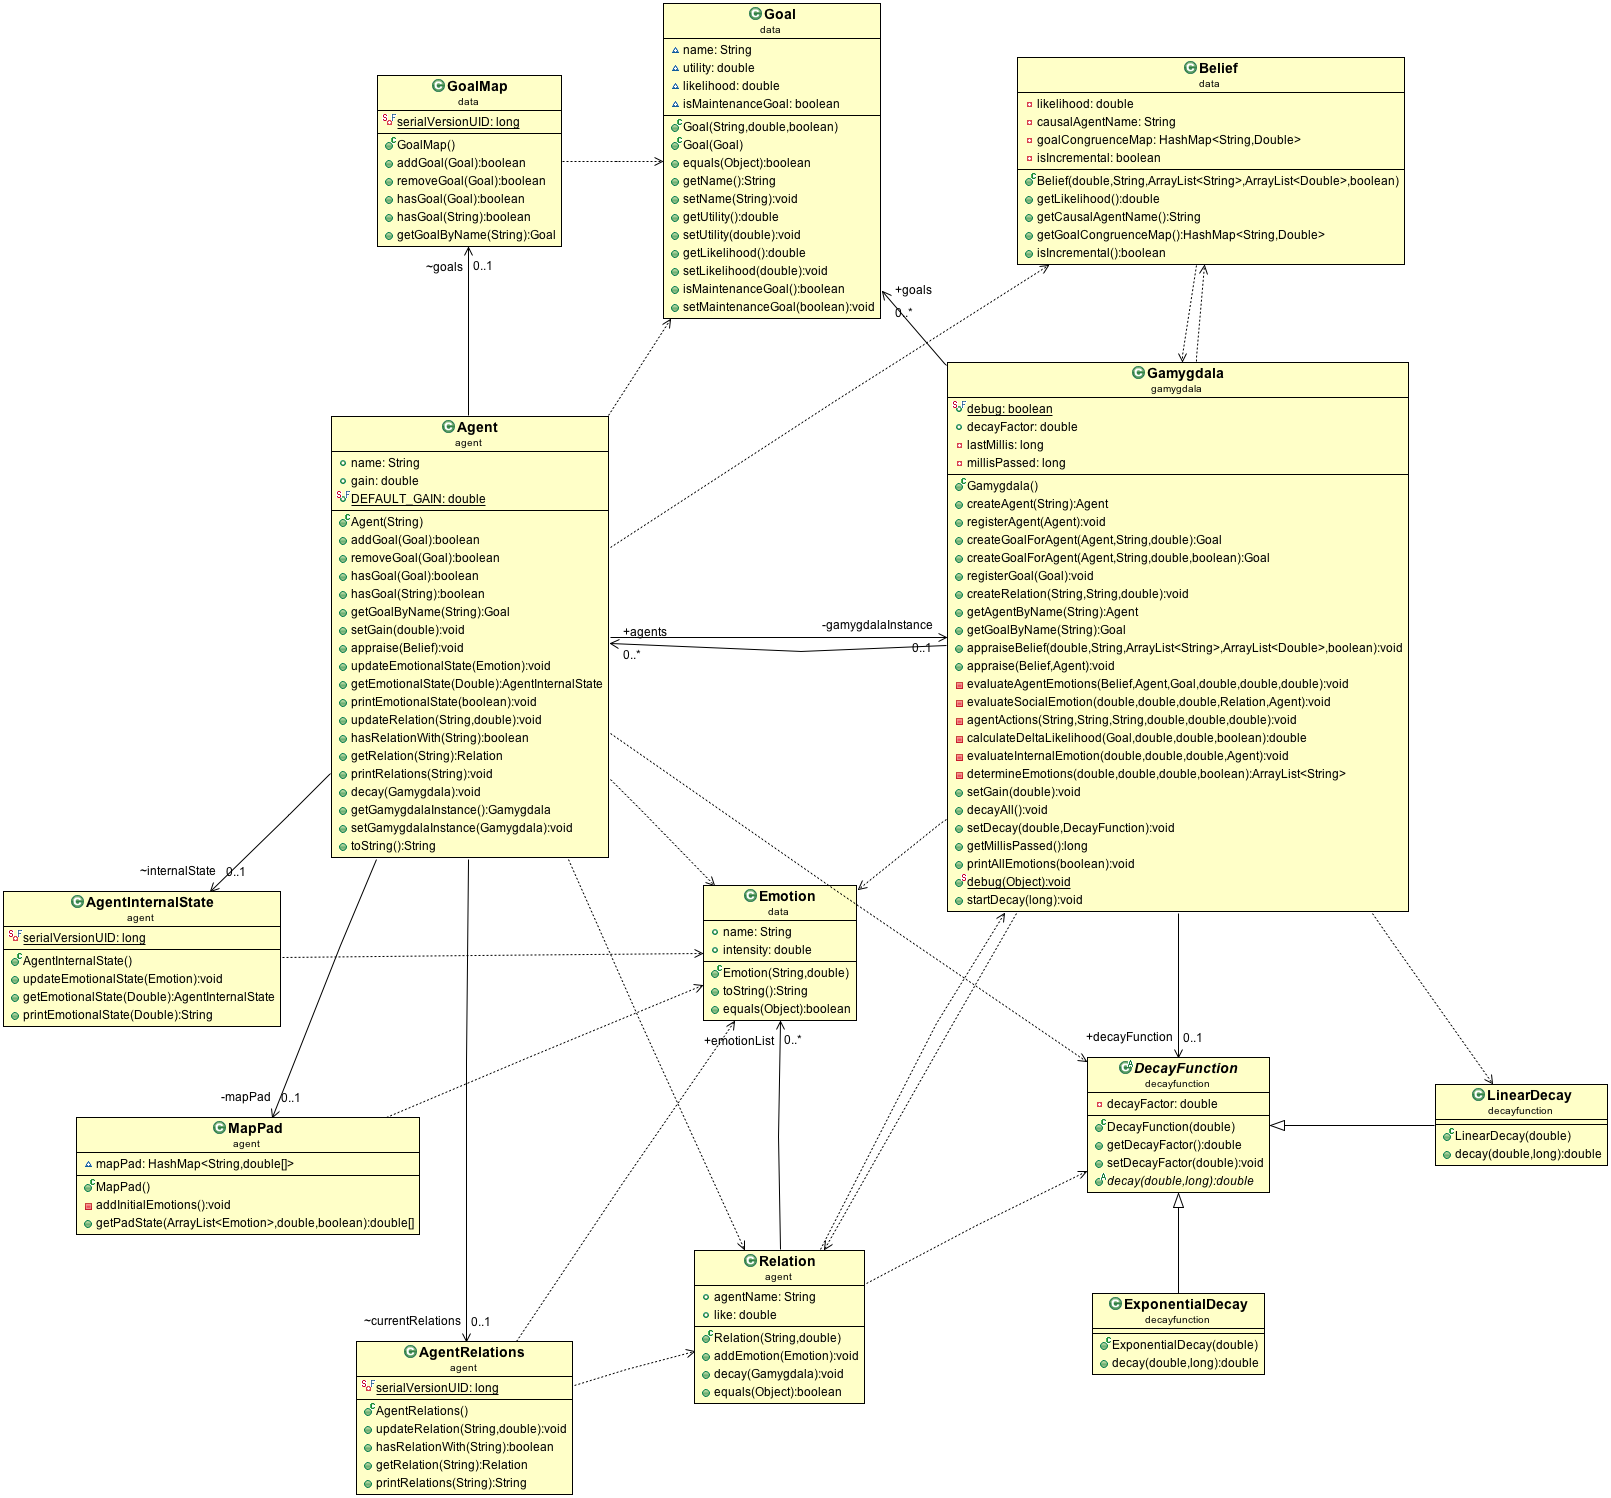
\includegraphics[width=\linewidth]{GAMYGDALA_UML_OLD}
\caption{The UML-diagram for the initial port.}
\end{figure}

\pagebreak

\begin{figure}
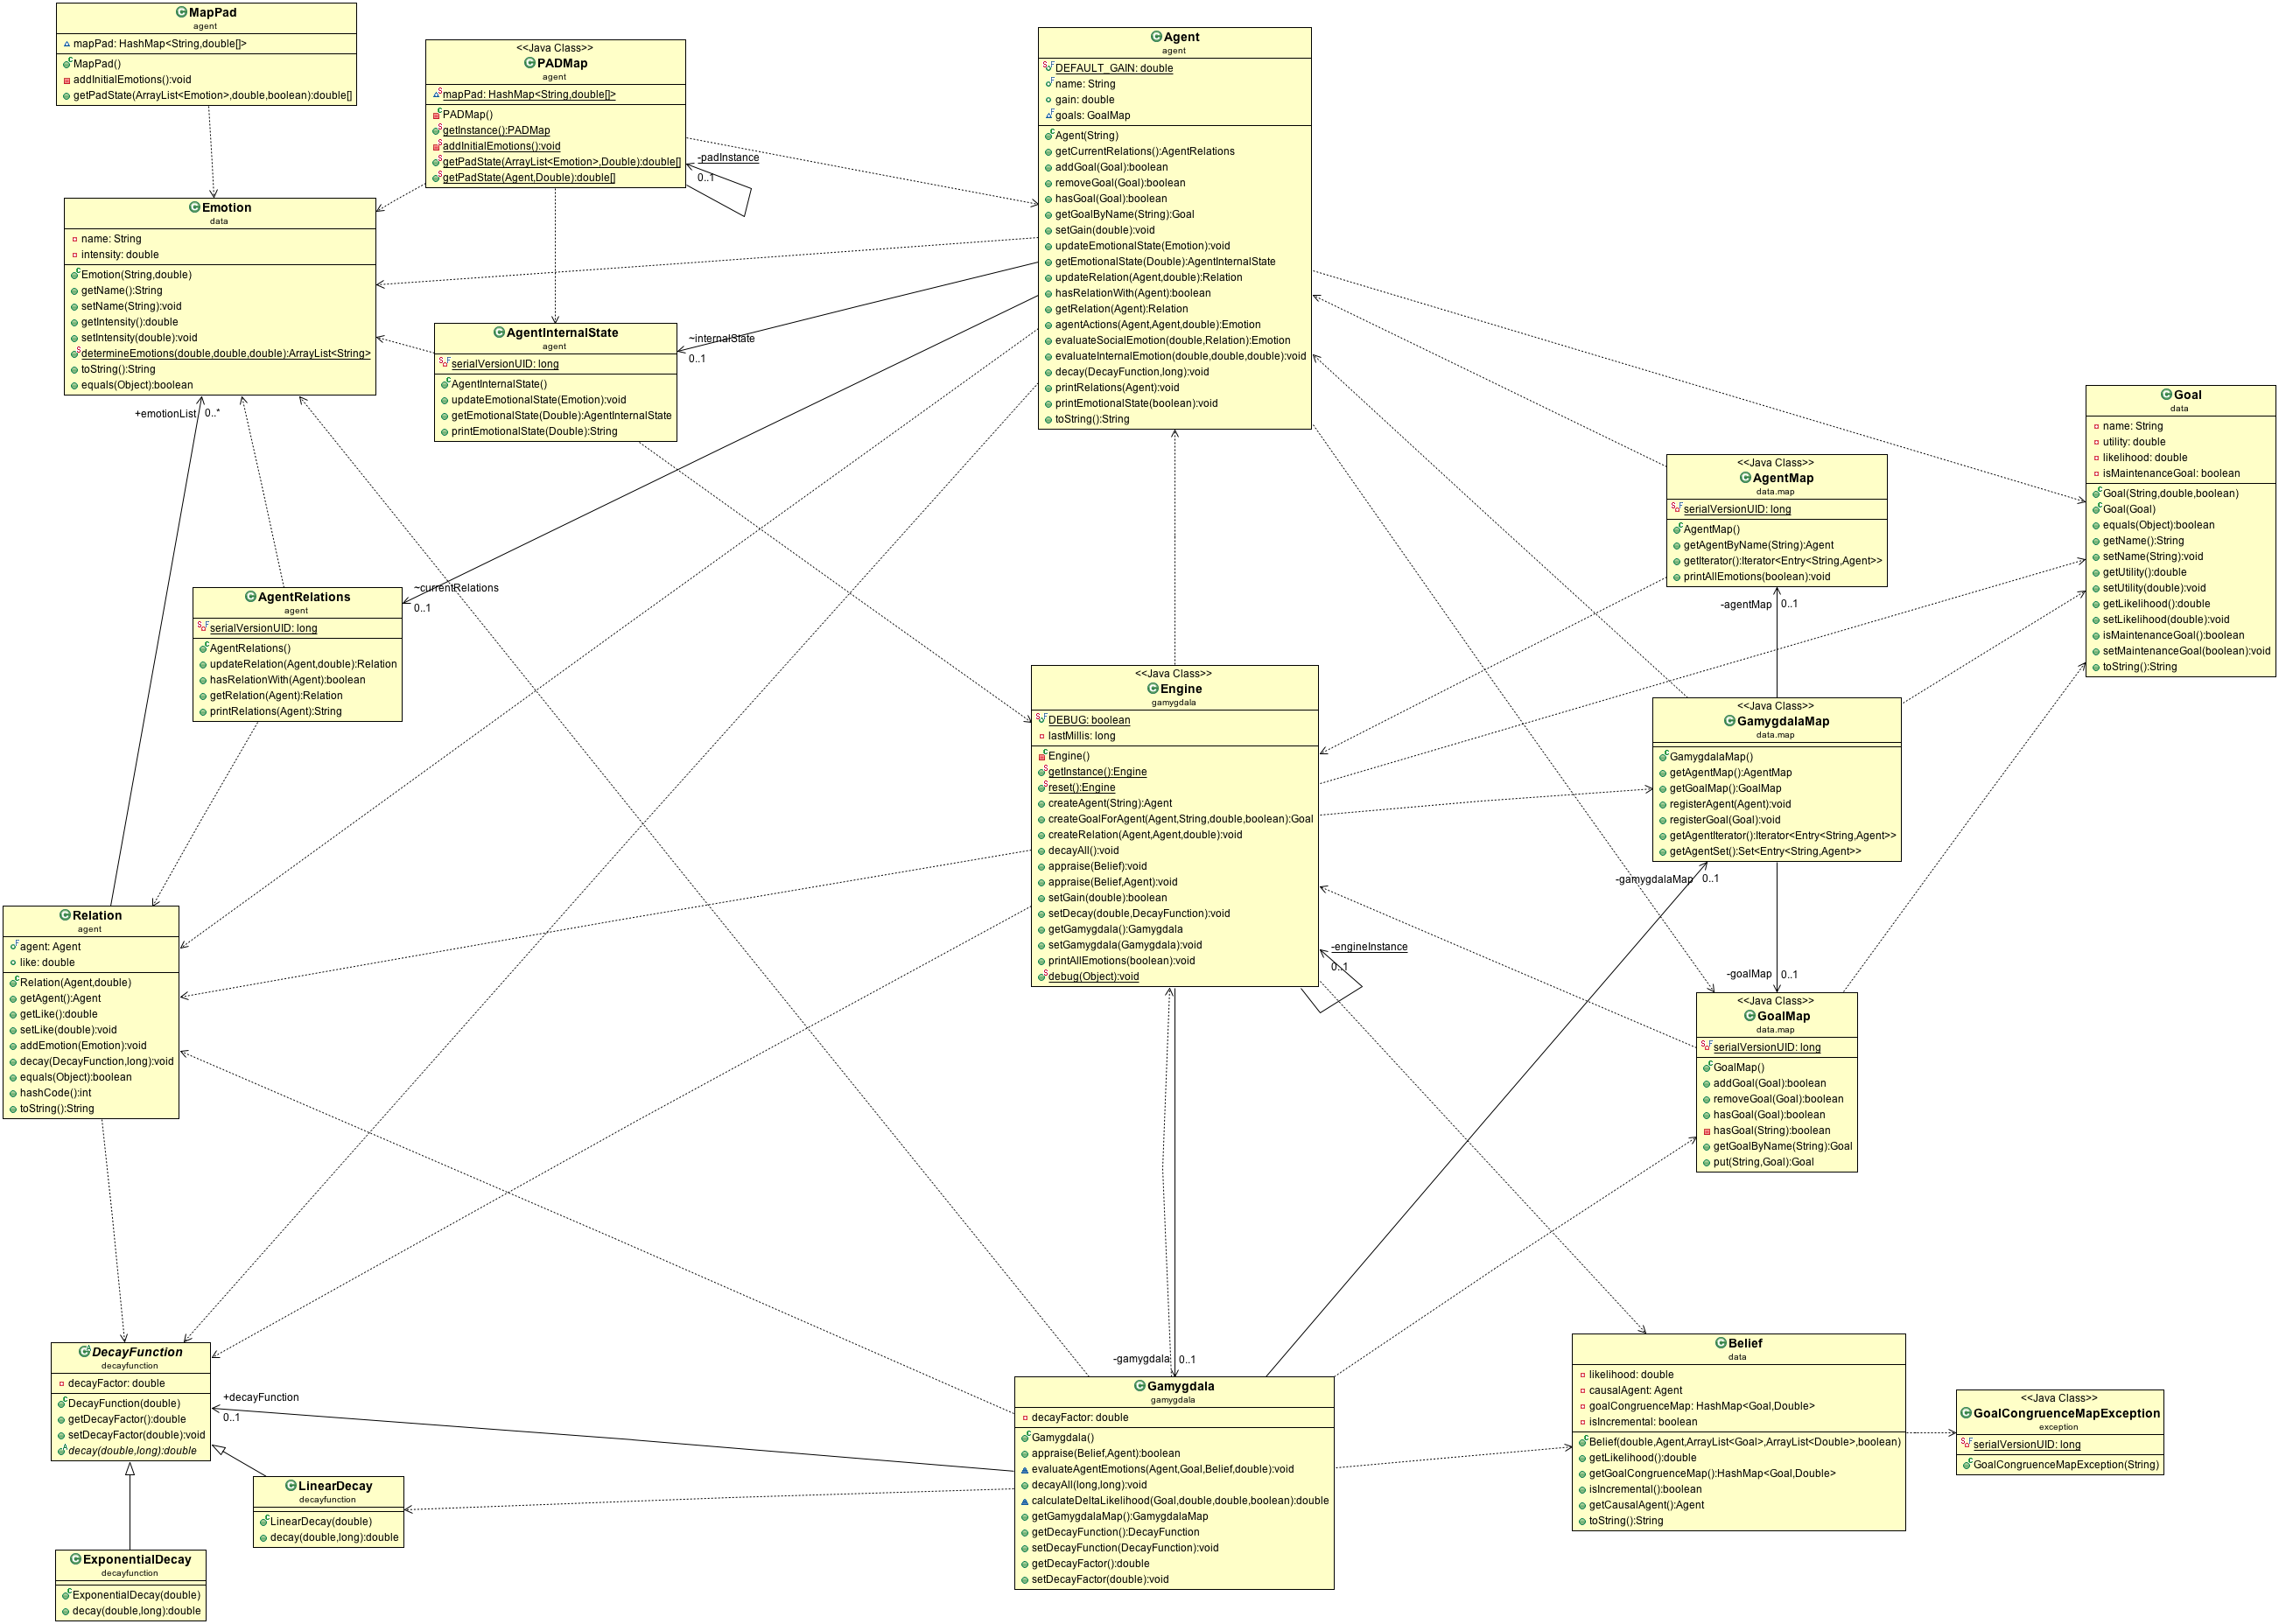
\includegraphics[width=\linewidth]{GAMYGDALA_UML_NEW}
\caption{The UML-diagram for the re-factored port.}
\end{figure}

\pagebreak

\subsection{GAMYGDALA Emergent Architecture}
This project aims to create a good GAMYGDALA port in Java. With that in mind you could say that the architectural design was not emergent, because the original GAMYGDALA already had an architecture. But this is not true. Porting from JavaScript to Java brings a lot of needed creativity with it. For example JavaScript works mostly with String and Java with objects, this transition was a real brainteaser. To implement better software engineering methods, the architecture of the port needed to emerge, but the function needed to stay the same. We ensured this with the following actions: unit testing, benchmark testing and re-factoring. 

\subsubsection{Testing}
Testing is one of the most important software engineering aspects. Especially for a port is testing very important, because the port needs to work exactly the same as the original program. To make sure the port works exactly the same, we made use of two different types of testing. The first is Unit testing, and the second is a Benchmark.

	\subparagraph{Unit testing}
A Unit test determines whether a method still functions the same as intended to do. After the initial port, useful unit tests were made to ensure the purpose of the functions. After every re-factored piece of method, running the unit tests made sure that the method still functioned the same. By this way of testing there were some bugs found in the new code after we did the re-factor.

	\subparagraph{Benchmark testing}
Benchmark testing was very important for this system. A benchmark tests whether your whole programs functions like it was intended to do. If the right Emotions where calculated when certain Goals and Beliefs where added to the Engine. And whether certain relations where made when a Goal belongs to another Agent, but it affected the other. After a successful benchmark test, the system is functionally correct. 

\subsubsection{Re-factoring}
After the initial port and re-factoring of GAMYGDALA, we came to the conclusion that the Java code was still not very pretty. It had long functions, big classes and still classes with multiple responsibilities. To counter these faults, we started a big re-factor of the code. First we divided some functions in smaller new functions with less responsibility. We distributed the smaller functions over different classes. These changes made the bigger classes smaller and gave them less responsibilities.  

\subsection{Design patterns}
Within the GAMYGDALA port there are several design patterns used. These patterns help to improve the code and make it easier to use and develop. In the following subsections, we will present to you the design patterns used within the code.

	\subsubsection{Singleton pattern}
The singleton pattern is very useful in cases where you want to have at most 1 object 	of a class. The Engine Class has the singleton pattern build in. This is because it is not useful to have two GAMYGDALA engines running beside each other. Emotions can be calculated for each agent, and relation too. So there is no need for a second engine. It could only confuse programmers if they had accidentally created two different GAMYGDALA engines and has been working with both of them.  
  
	\subsubsection{Strategy pattern}
The strategy pattern is very useful when you have something that needs to be calculated and it depends on certain conditions how it needs to be calculated. Because of this we used the strategy pattern to determine the kind of emotions. The emotion calculation is based on the likelihood. For certain values of the likelihood there is a different strategy to calculate the kind of emotion.